\begin{comment}

In Figures \ref{fig:lasso_GLK_1}, \ref{fig:lasso_DEF_1}, \ref{fig:lasso_MID_1} and \ref{fig:lasso_FWD_1} the RMSE of the test set is plotted against different values of log($\lambda$) for goalkeepers, defenders, midfielders and forwards respectively. Further, their significant variables are listed in Tables \ref{tab:sig_var_GLK_1}, \ref{tab:sig_var_DEF_1}, \ref{tab:sig_var_MID_1} and \ref{tab:sig_var_FWD_1} respectively.

\end{comment}

\begin{comment}


\begin{figure}[H]
    \centering
    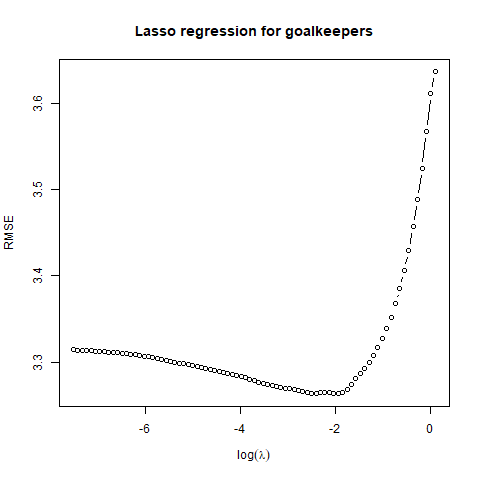
\includegraphics[scale=0.55]{fig/chapter_6/lasso_GLK.png}
    \caption{RMSE for different values of $\lambda$ for goalkeepers}
\label{fig:lasso_GLK}    
\end{figure}


\begin{table}[H]
\centering
\caption{Significant Variables for goalkeepers based on lasso regression and RMSE}
\label{tab:sig_var_GLK}
\begin{tabular}{l}
\textbf{Significant variables for goalkeepers }\\
Opponent                              \\
Team                                  \\
Cost                                  \\
Transfers in                          \\
Transfers out                         \\
Home/Away                             \\
Minutes played                        \\
Saves                                 \\
Clean Sheets                          \\
Assists                               \\
Own Goals                            
\end{tabular}
\end{table}

\end{comment}


\begin{comment}
\begin{figure}
\centering
\begin{minipage}{.5\textwidth}
  \centering
  \captionsetup{justification=centering}
  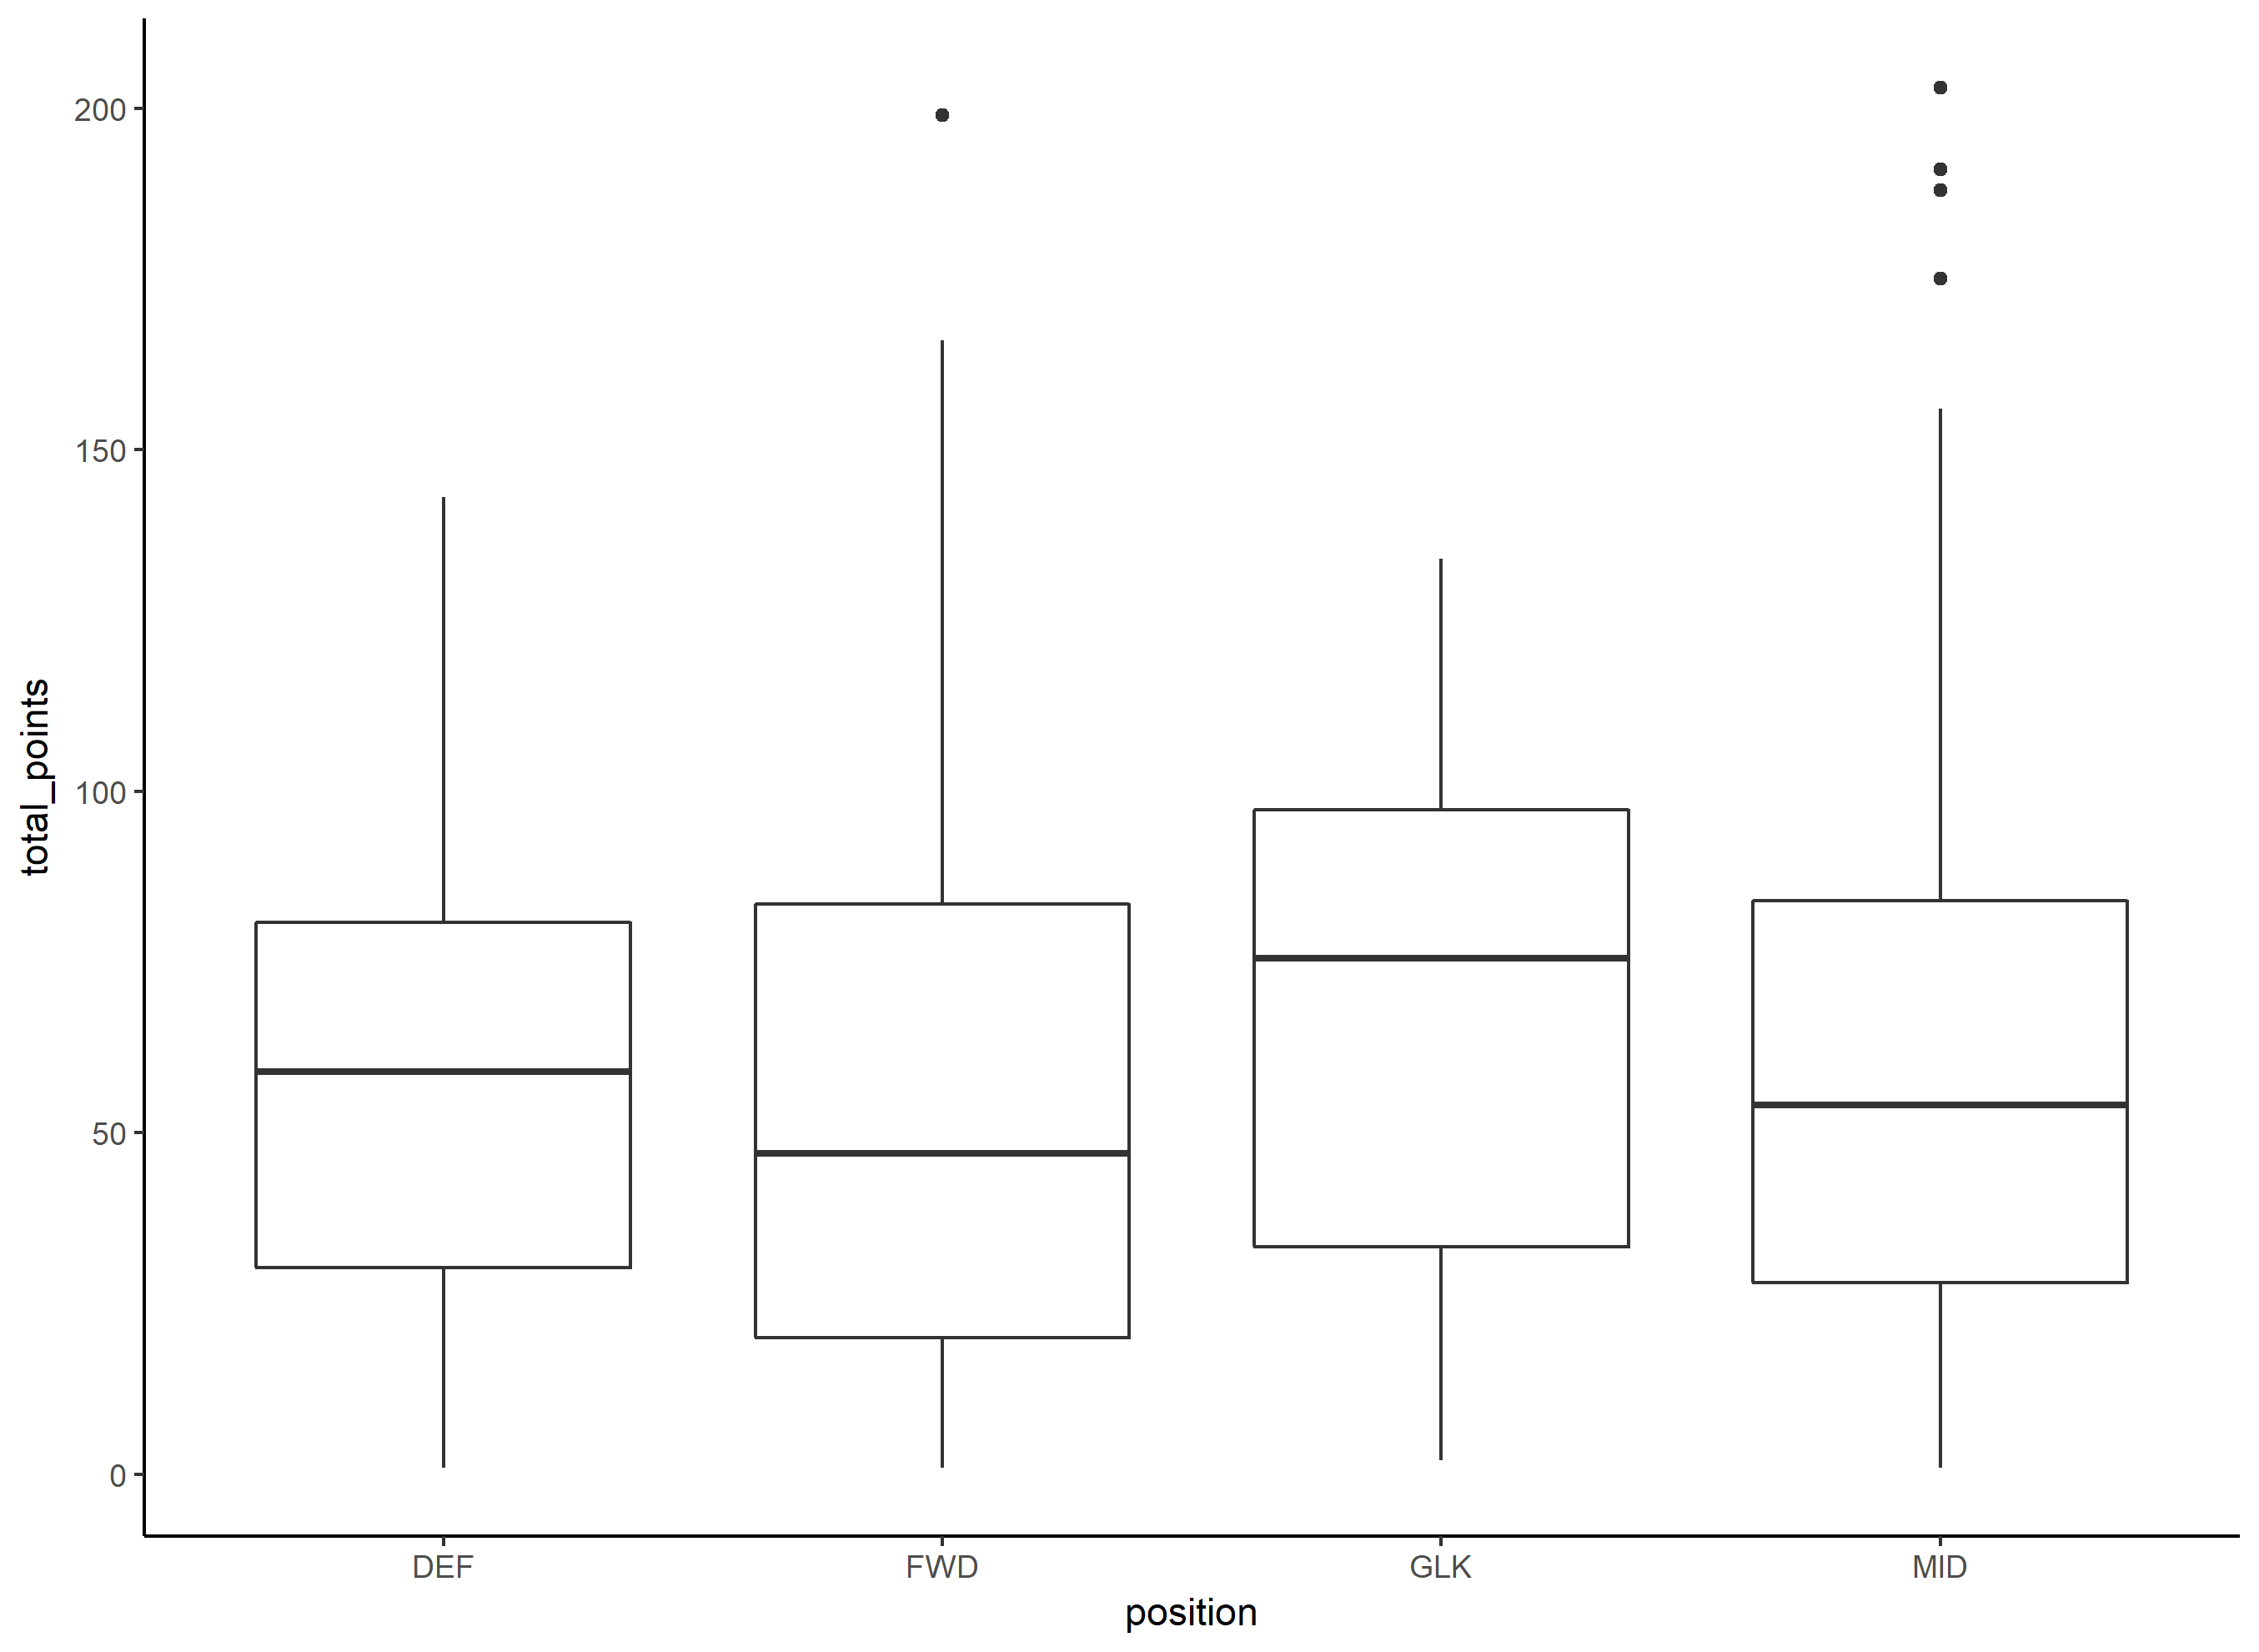
\includegraphics[width=.9\linewidth]{fig/chapter_6/box_plot_positions.png}
  \captionof{figure}{Box-plot of total points obtained in different positions over the 2016 season gameweek 1-32.}
  \label{fig:box_plot}
\end{minipage}%
\begin{minipage}{.5\textwidth}
  \centering
  \captionsetup{justification=centering}
  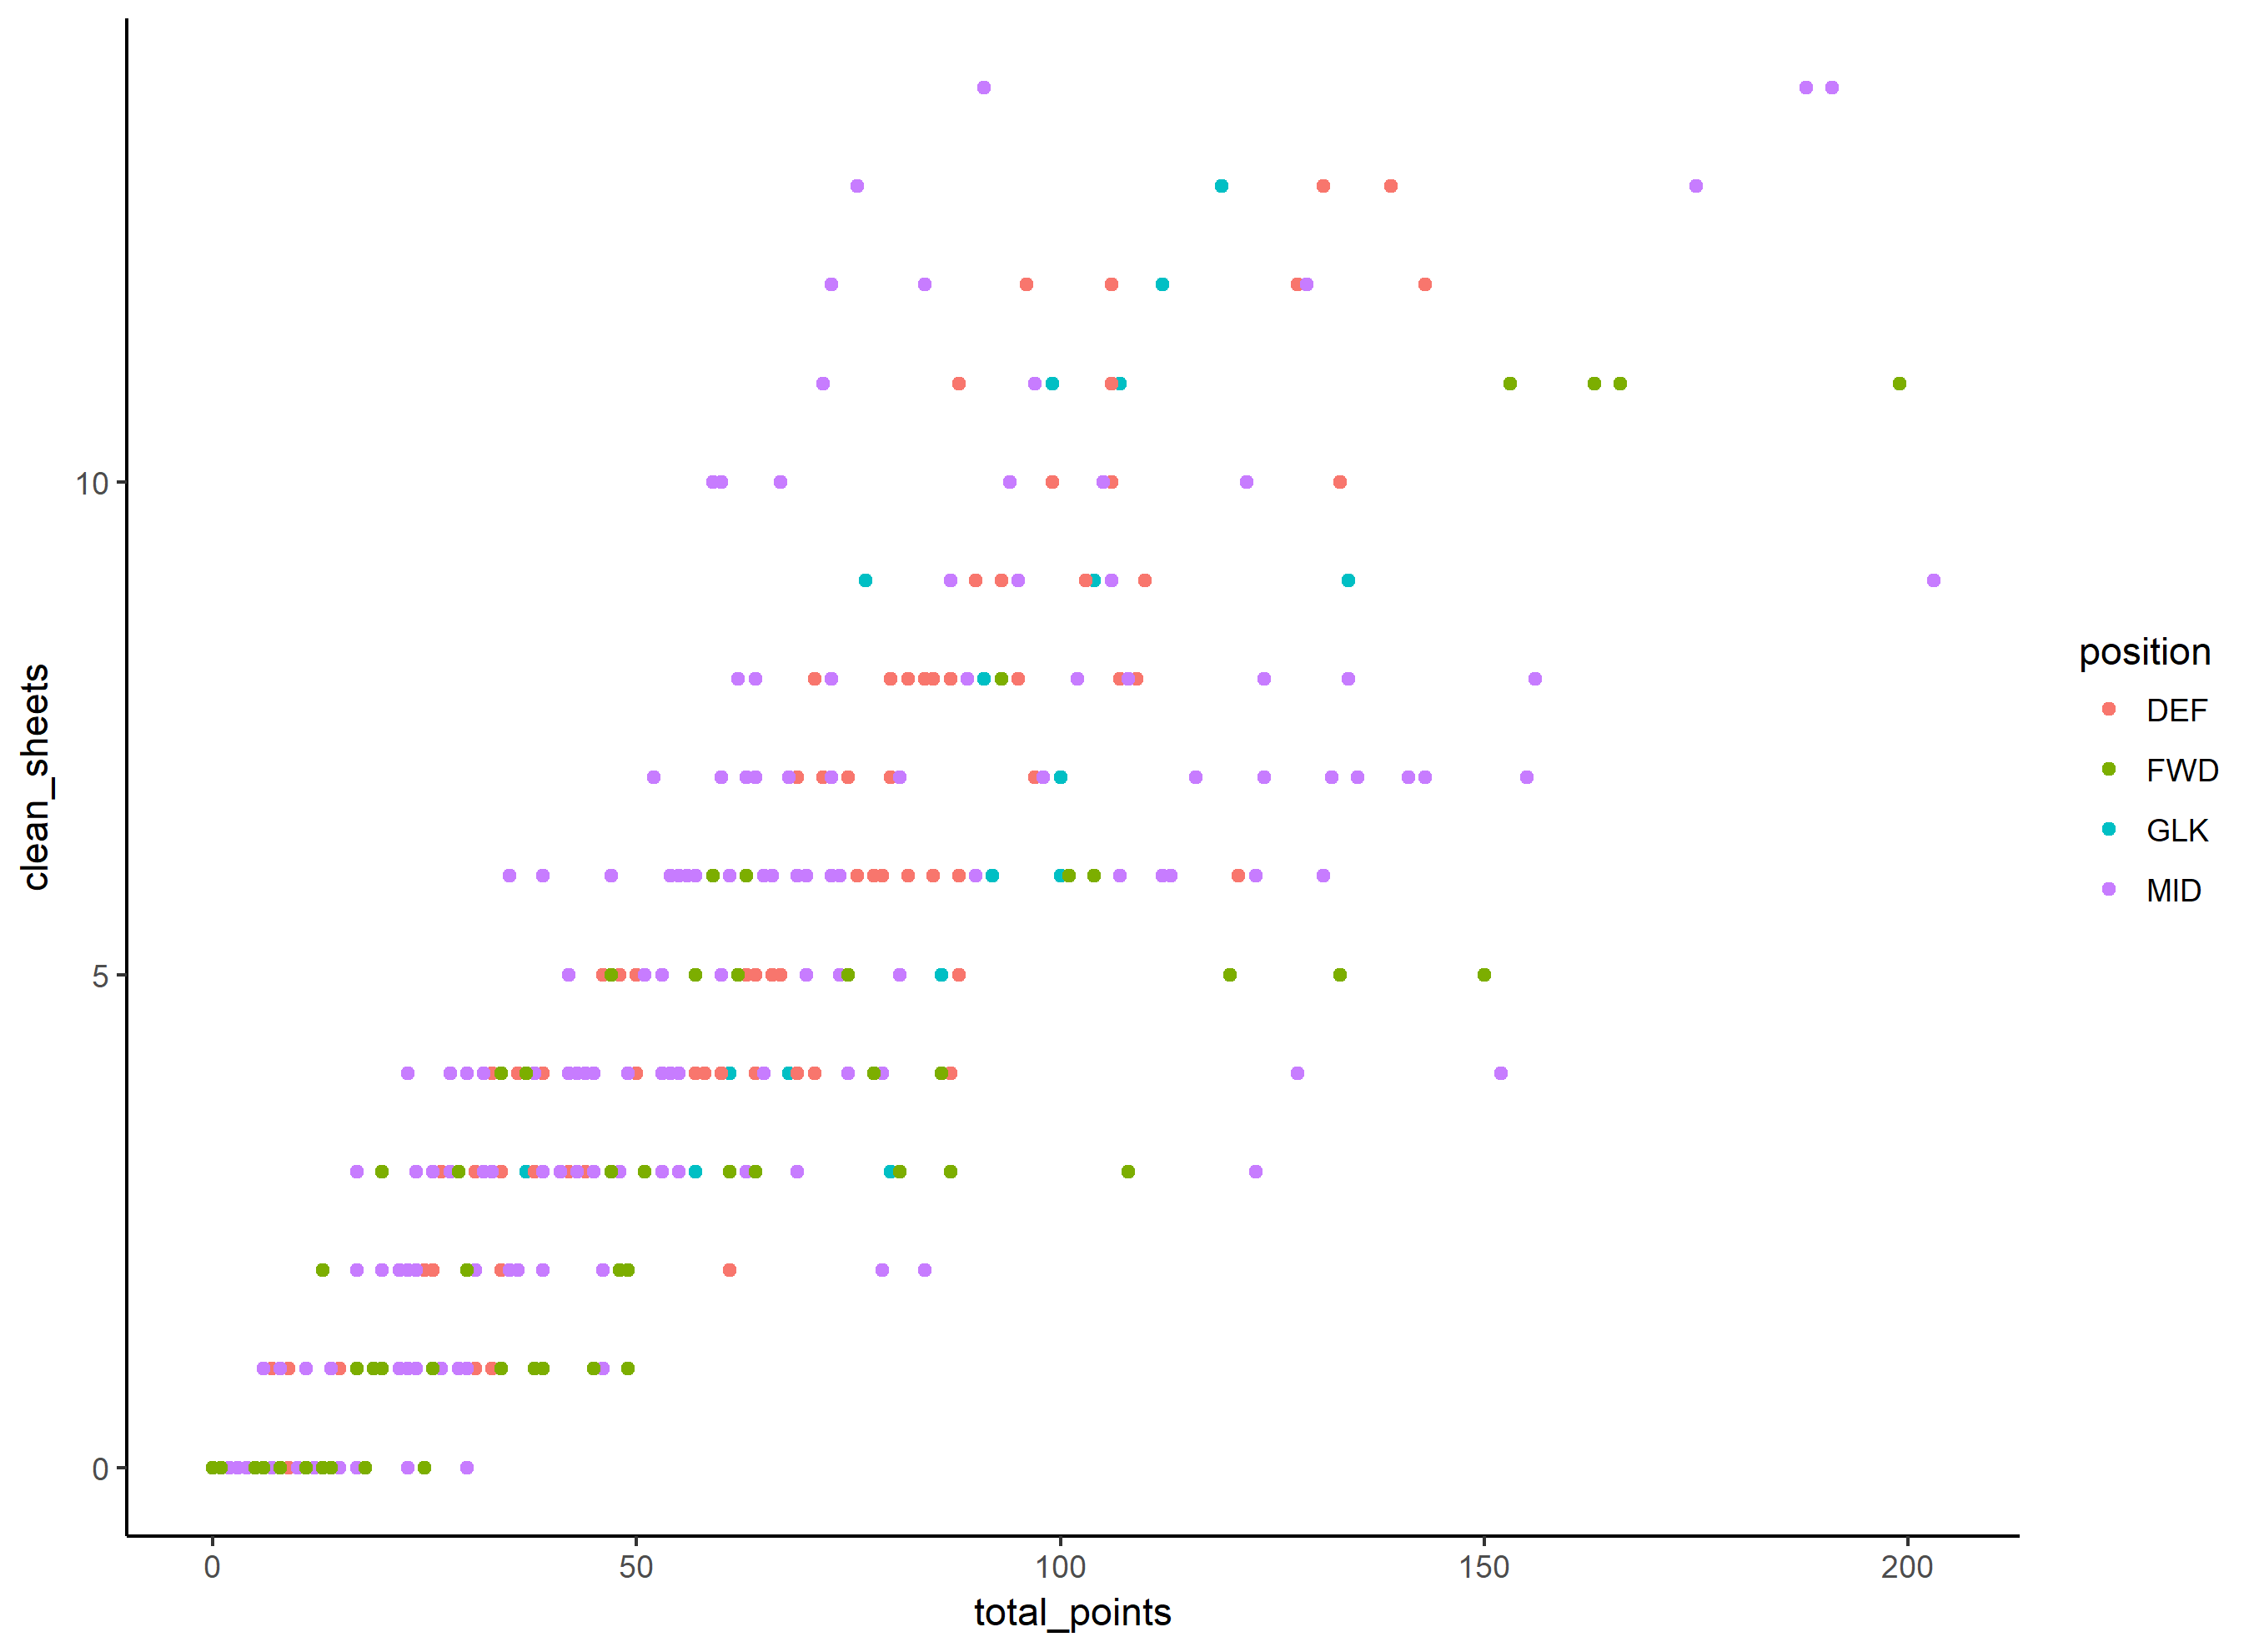
\includegraphics[width=.9\linewidth]{fig/chapter_6/clean_sheet_tot_poins.png}
  \captionof{figure}{Clean Sheets and Total points for different positions.}
  \label{fig:cs_tot_p}
\end{minipage}
\end{figure}

\begin{figure}[H]
\centering
\begin{subfigure}{.5\textwidth}
  \centering
  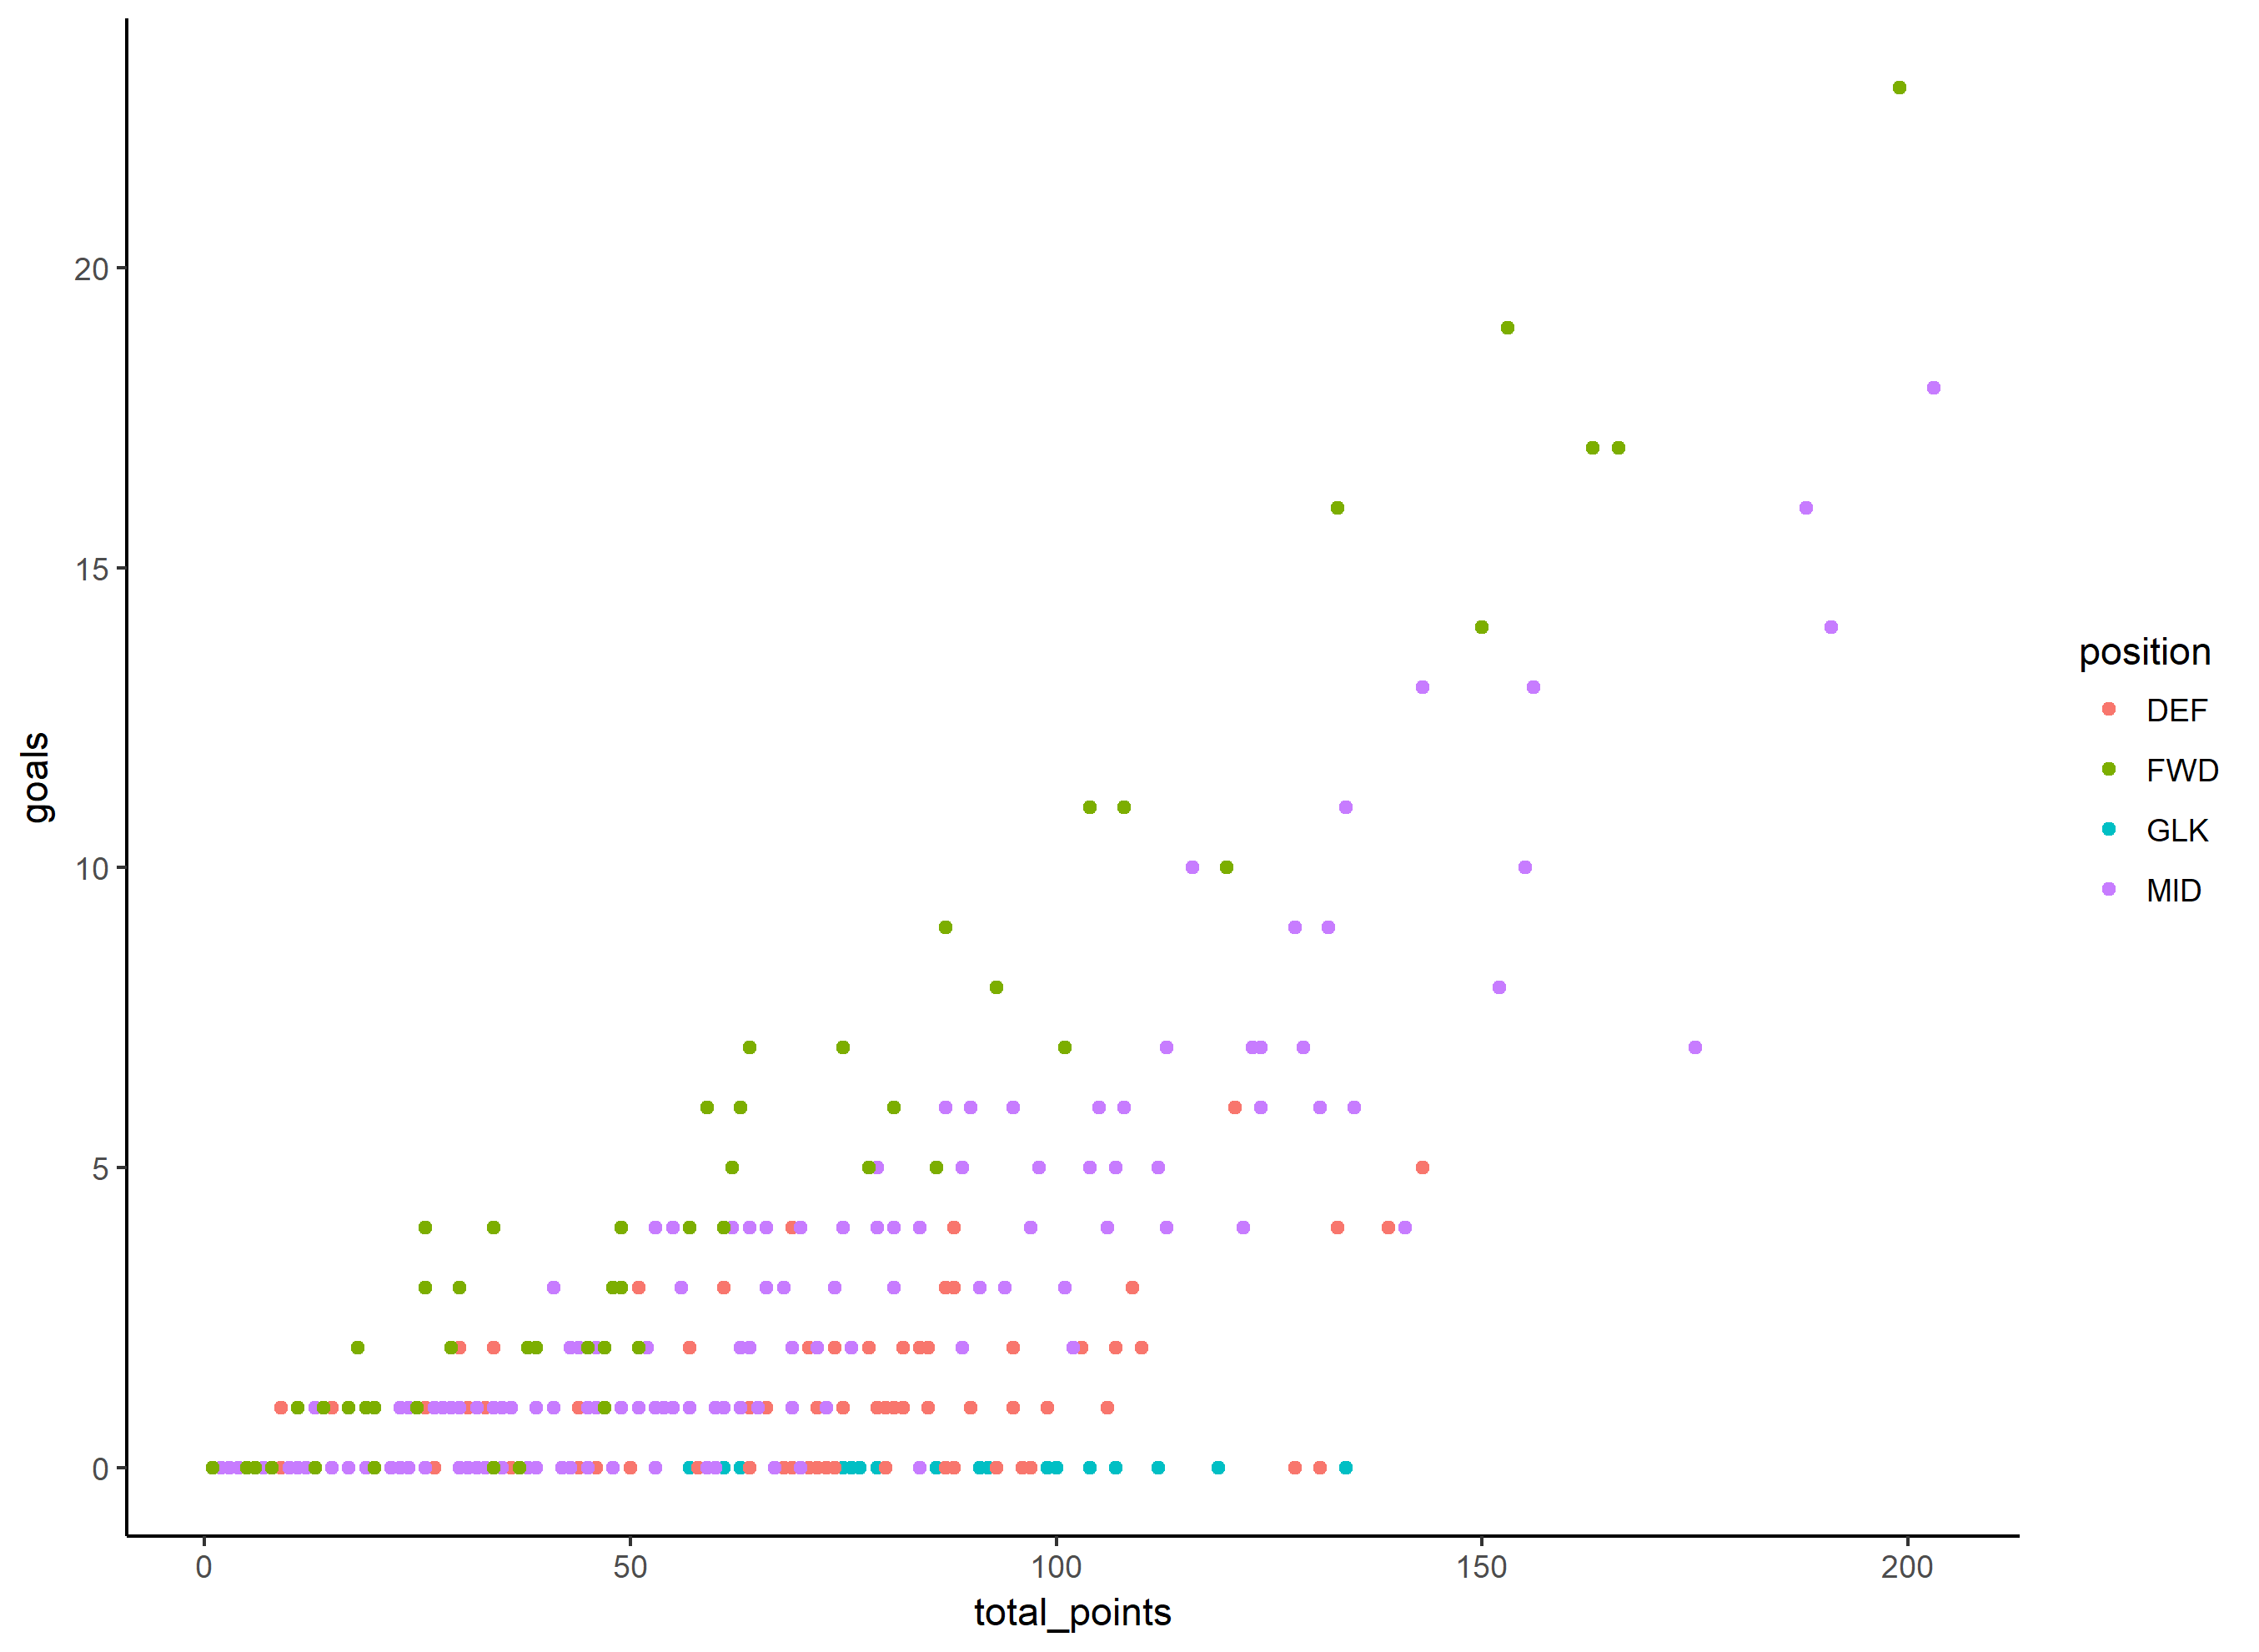
\includegraphics[width=.9\linewidth]{fig/chapter_6/goals_tot_poins.png}
  \caption{Goals and Total points for different positions.}
  \label{fig:goal_tot_p}
\end{subfigure}%
\begin{subfigure}{.5\textwidth}
  \centering
  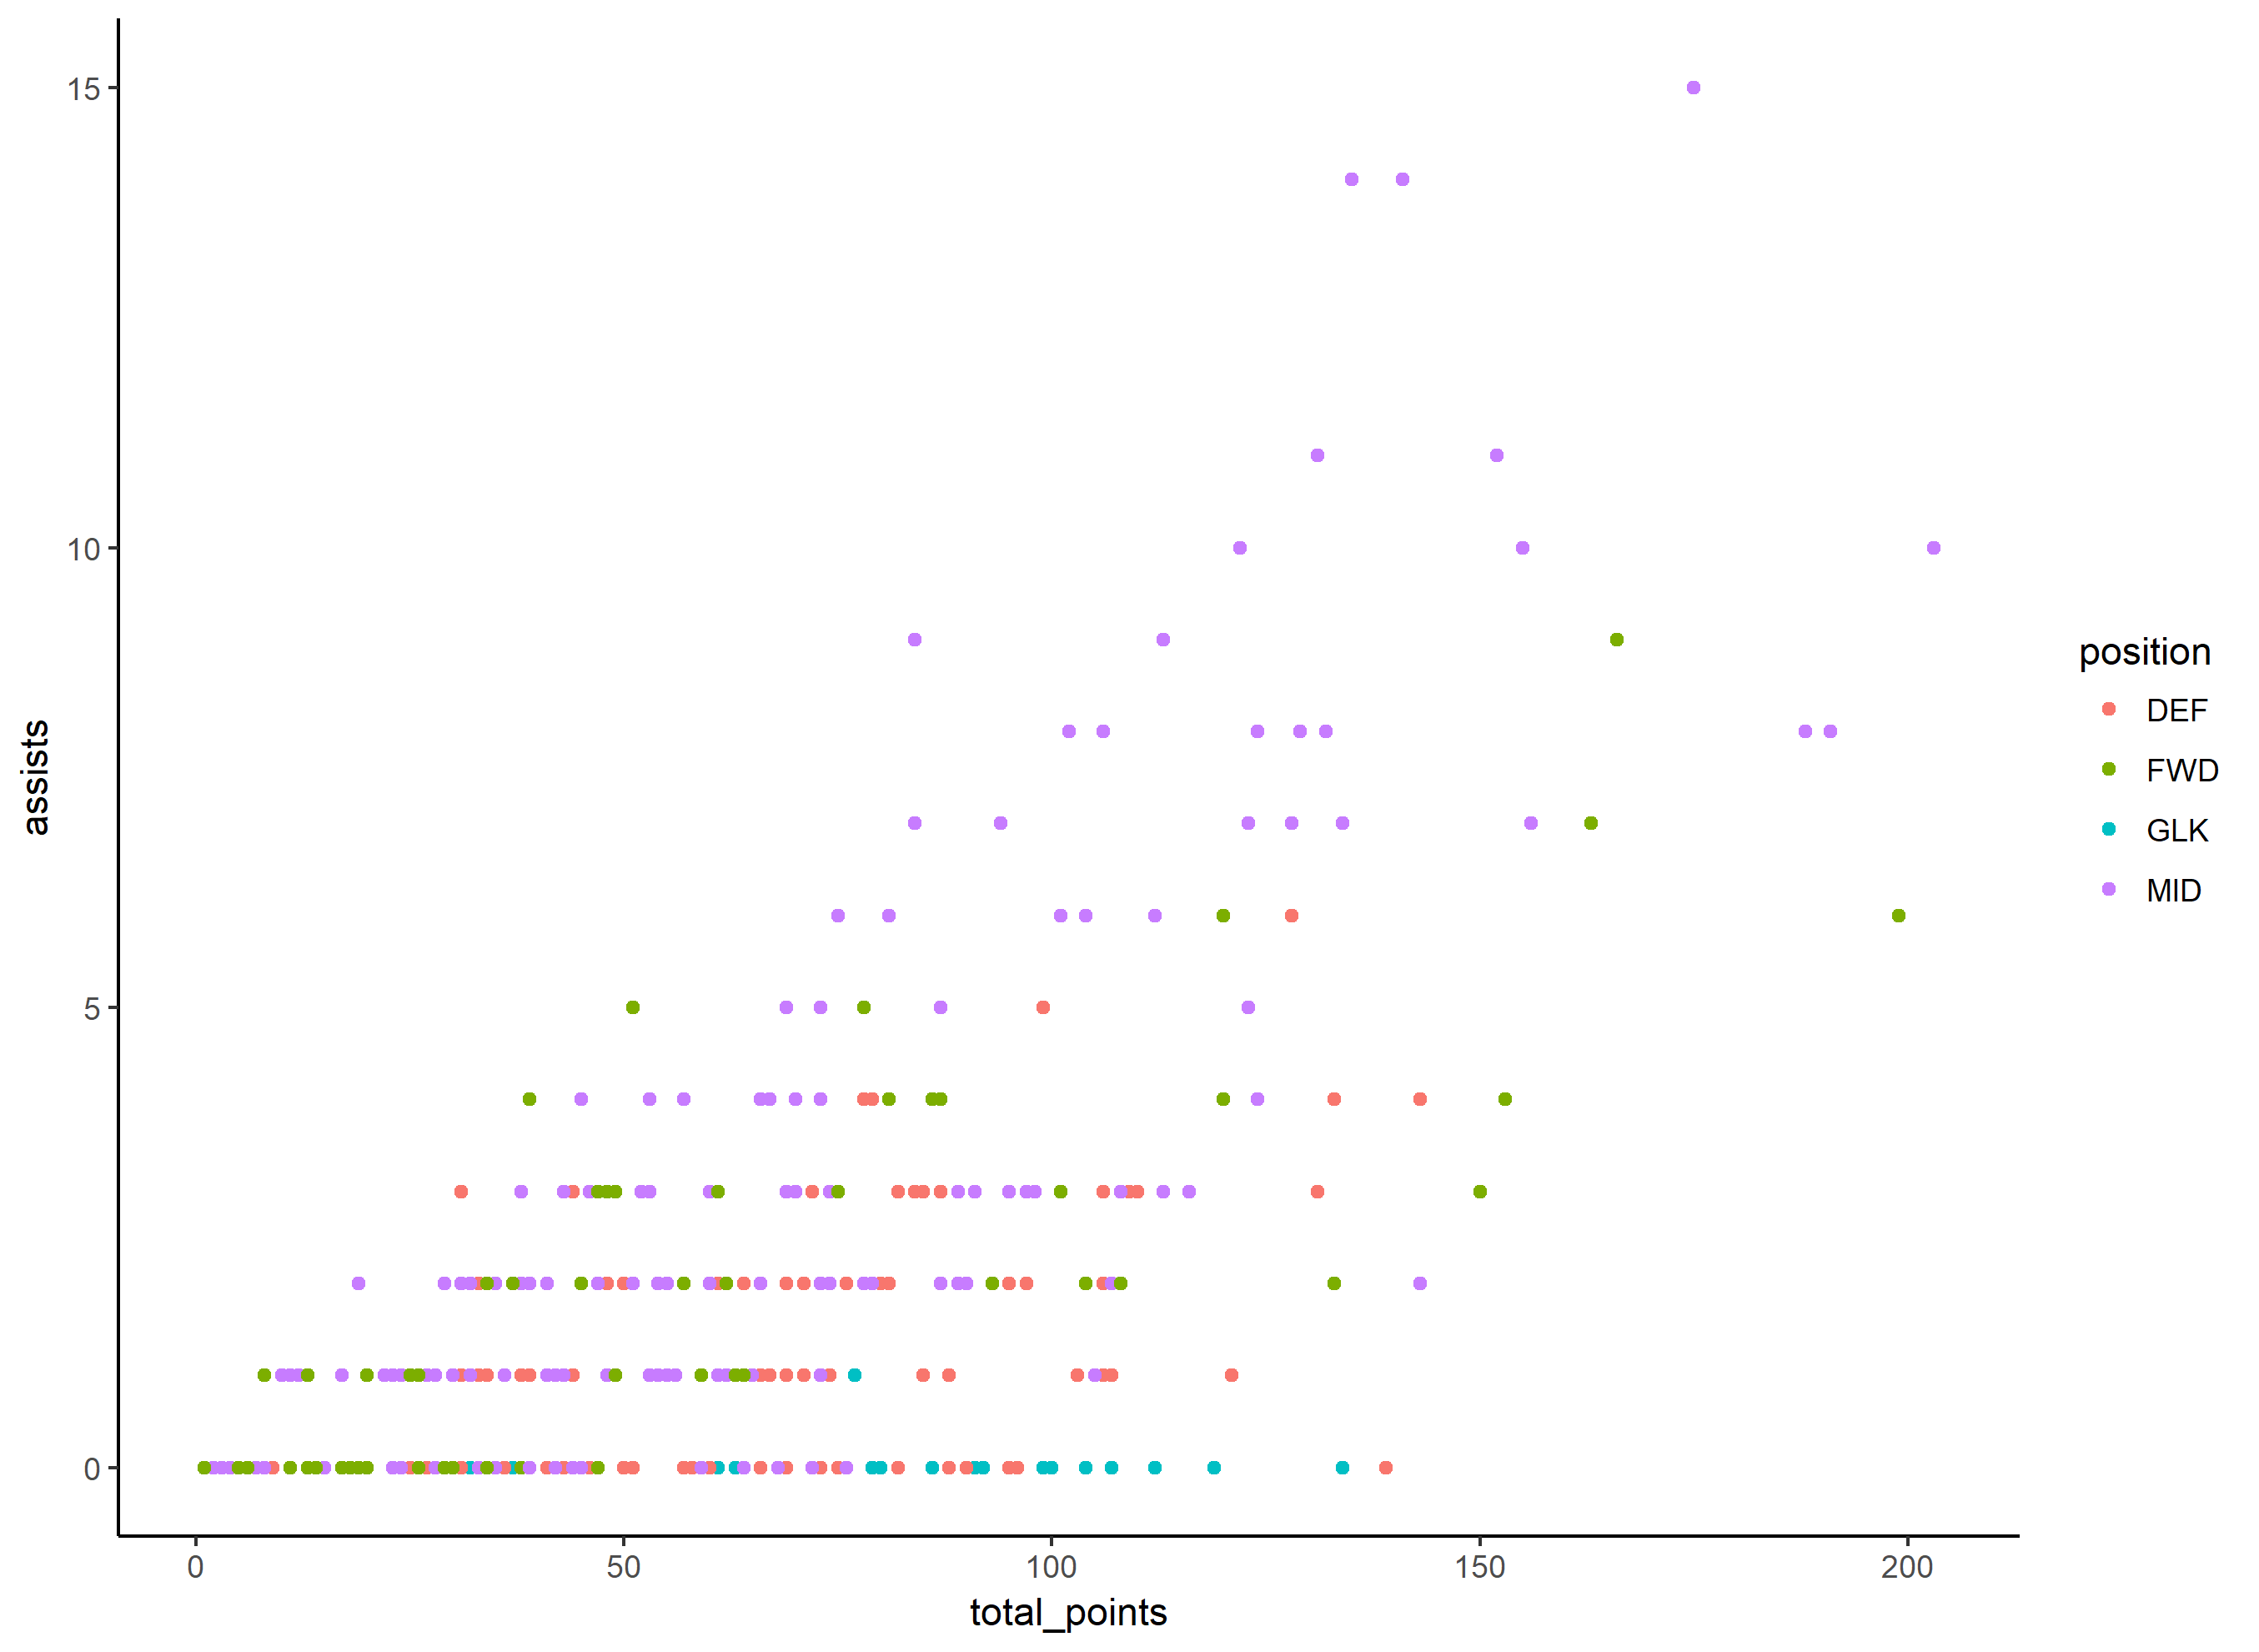
\includegraphics[width=.9\linewidth]{fig/chapter_6/assists_tot_poins.png}
  \caption{Time-series winter 16/17}
  \label{fig:assist_tot_p}
\end{subfigure}
\end{figure}




\begin{figure}[h!]
\centering
\begin{minipage}{.5\textwidth}
  \centering
  \captionsetup{justification=centering}
  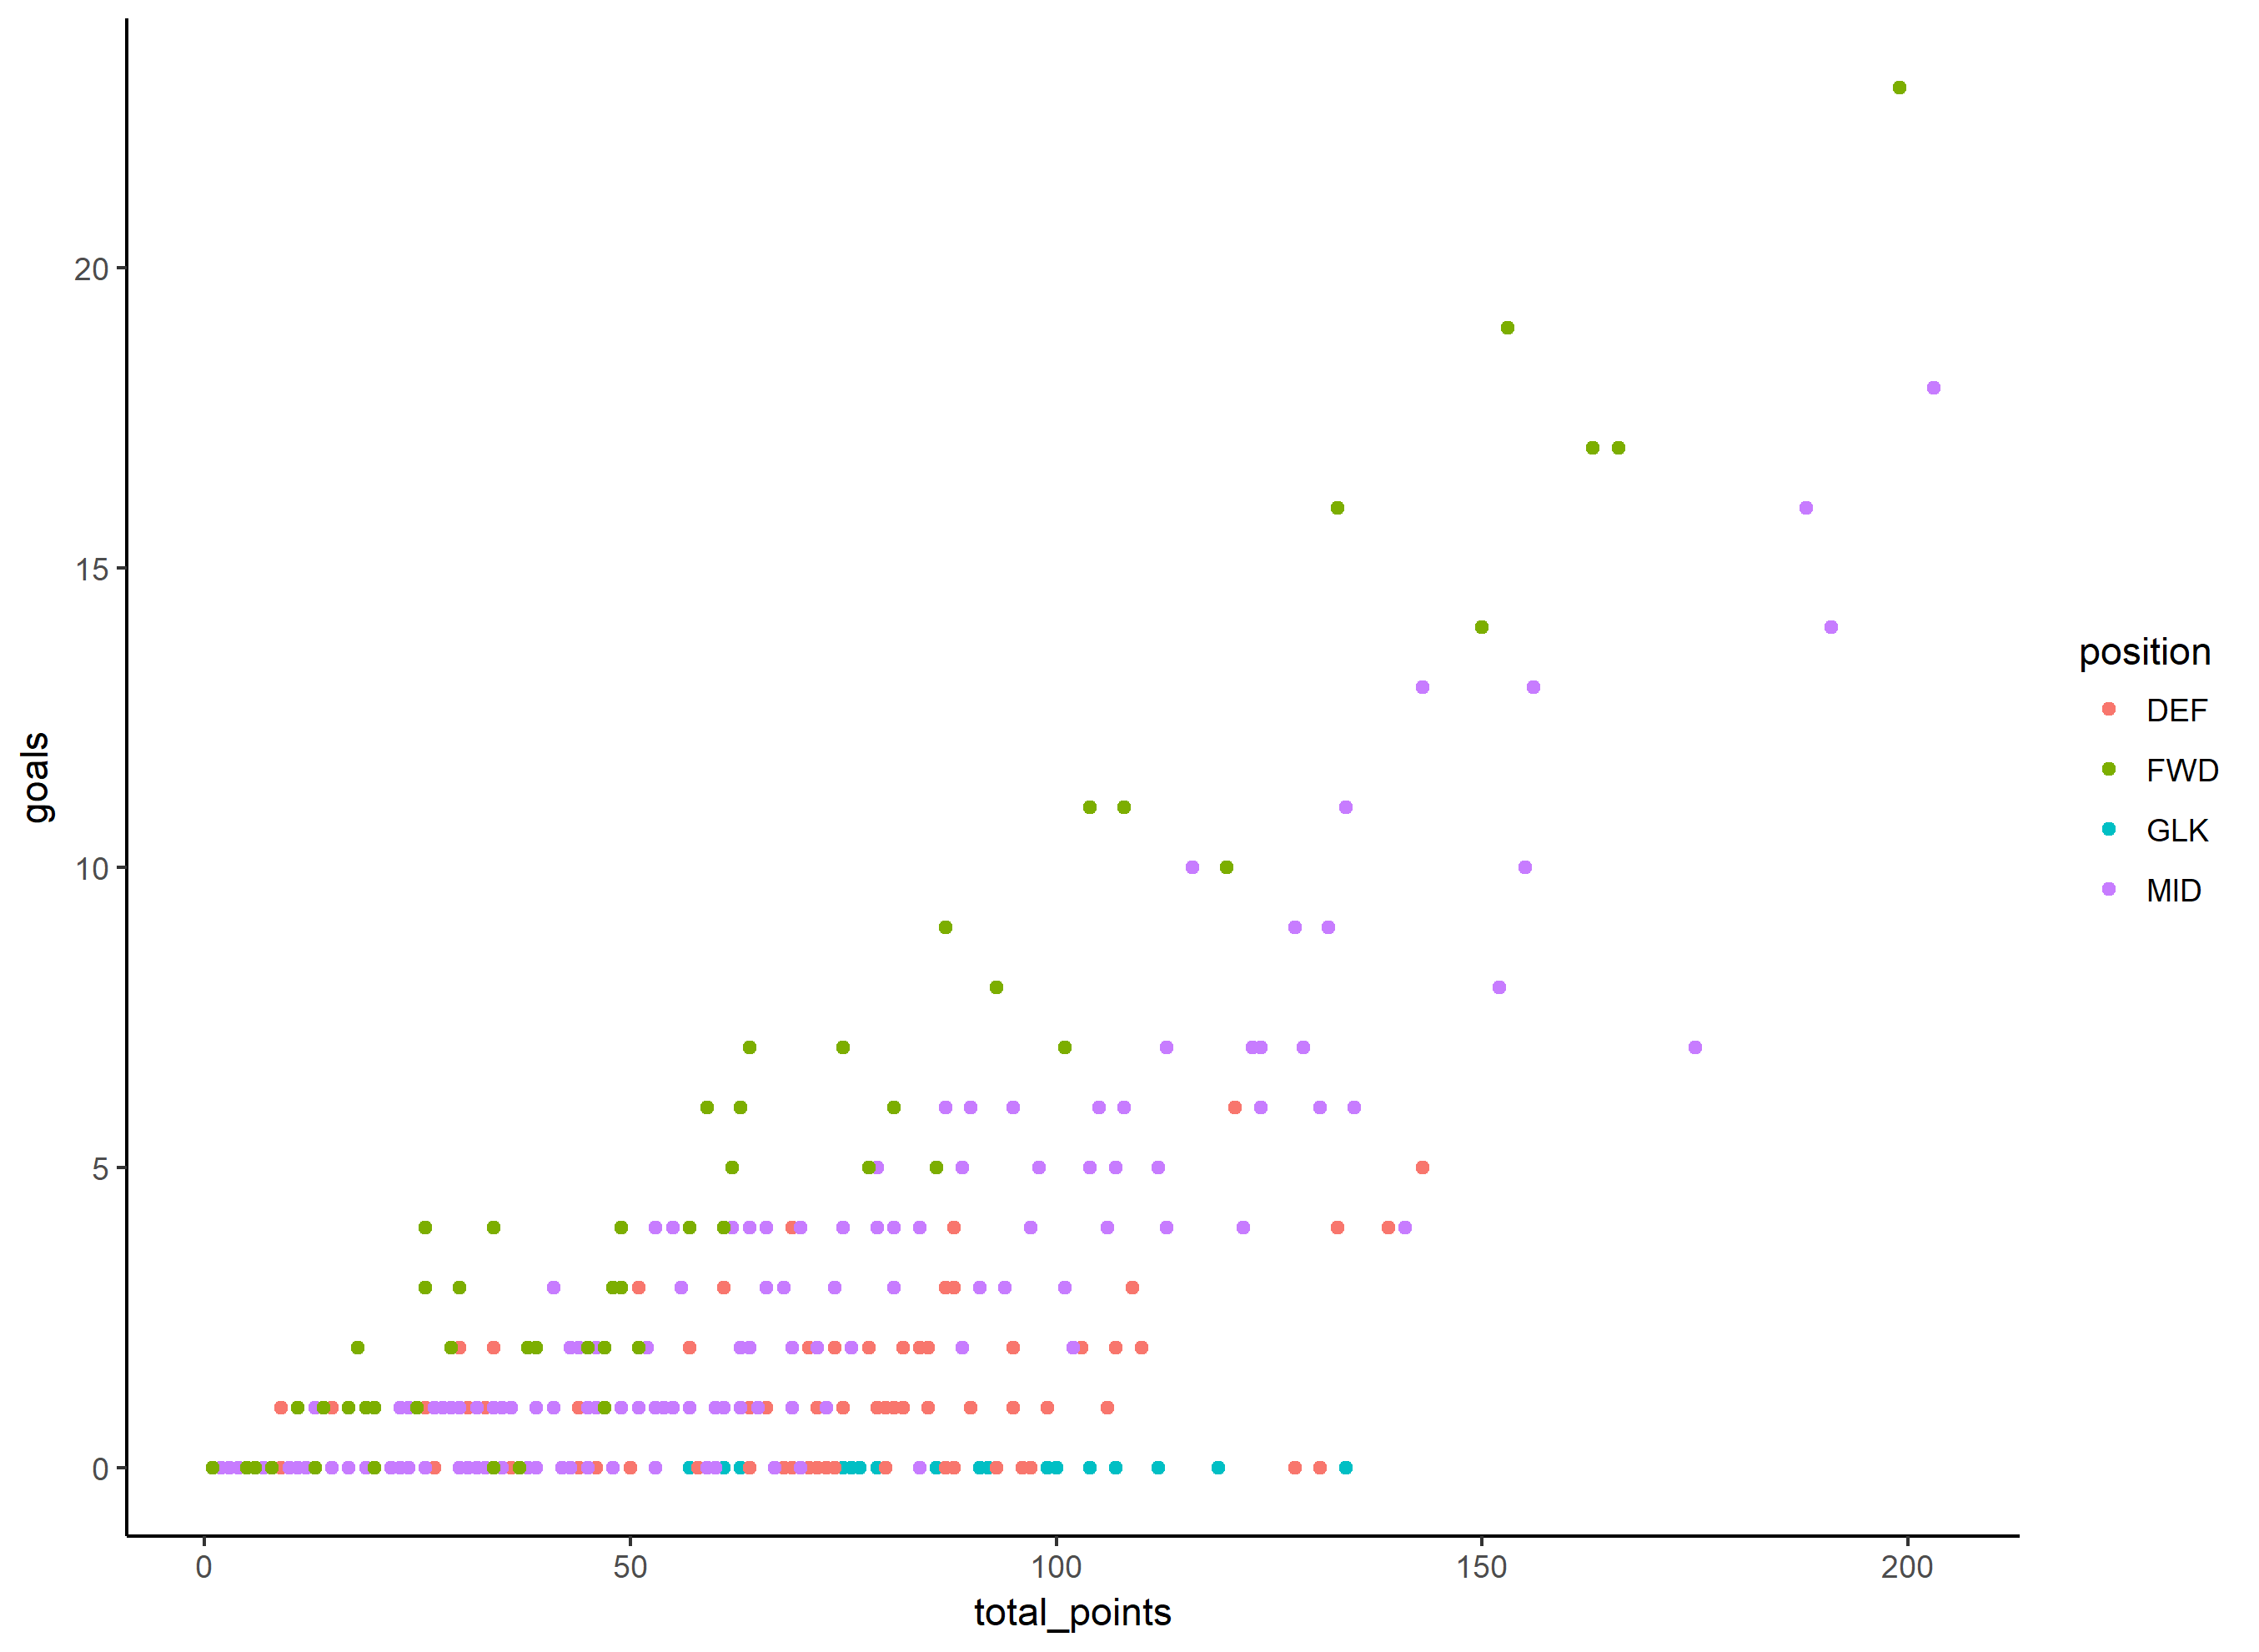
\includegraphics[width=.9\linewidth]{fig/chapter_6/goals_tot_poins.png}
  \caption{figure}{Goals and Total points for different positions.}
  \label{fig:goal_tot_p}
\end{minipage}
\hfill
\begin{minipage}{.5\textwidth}
  \centering
  \captionsetup{justification=centering}
  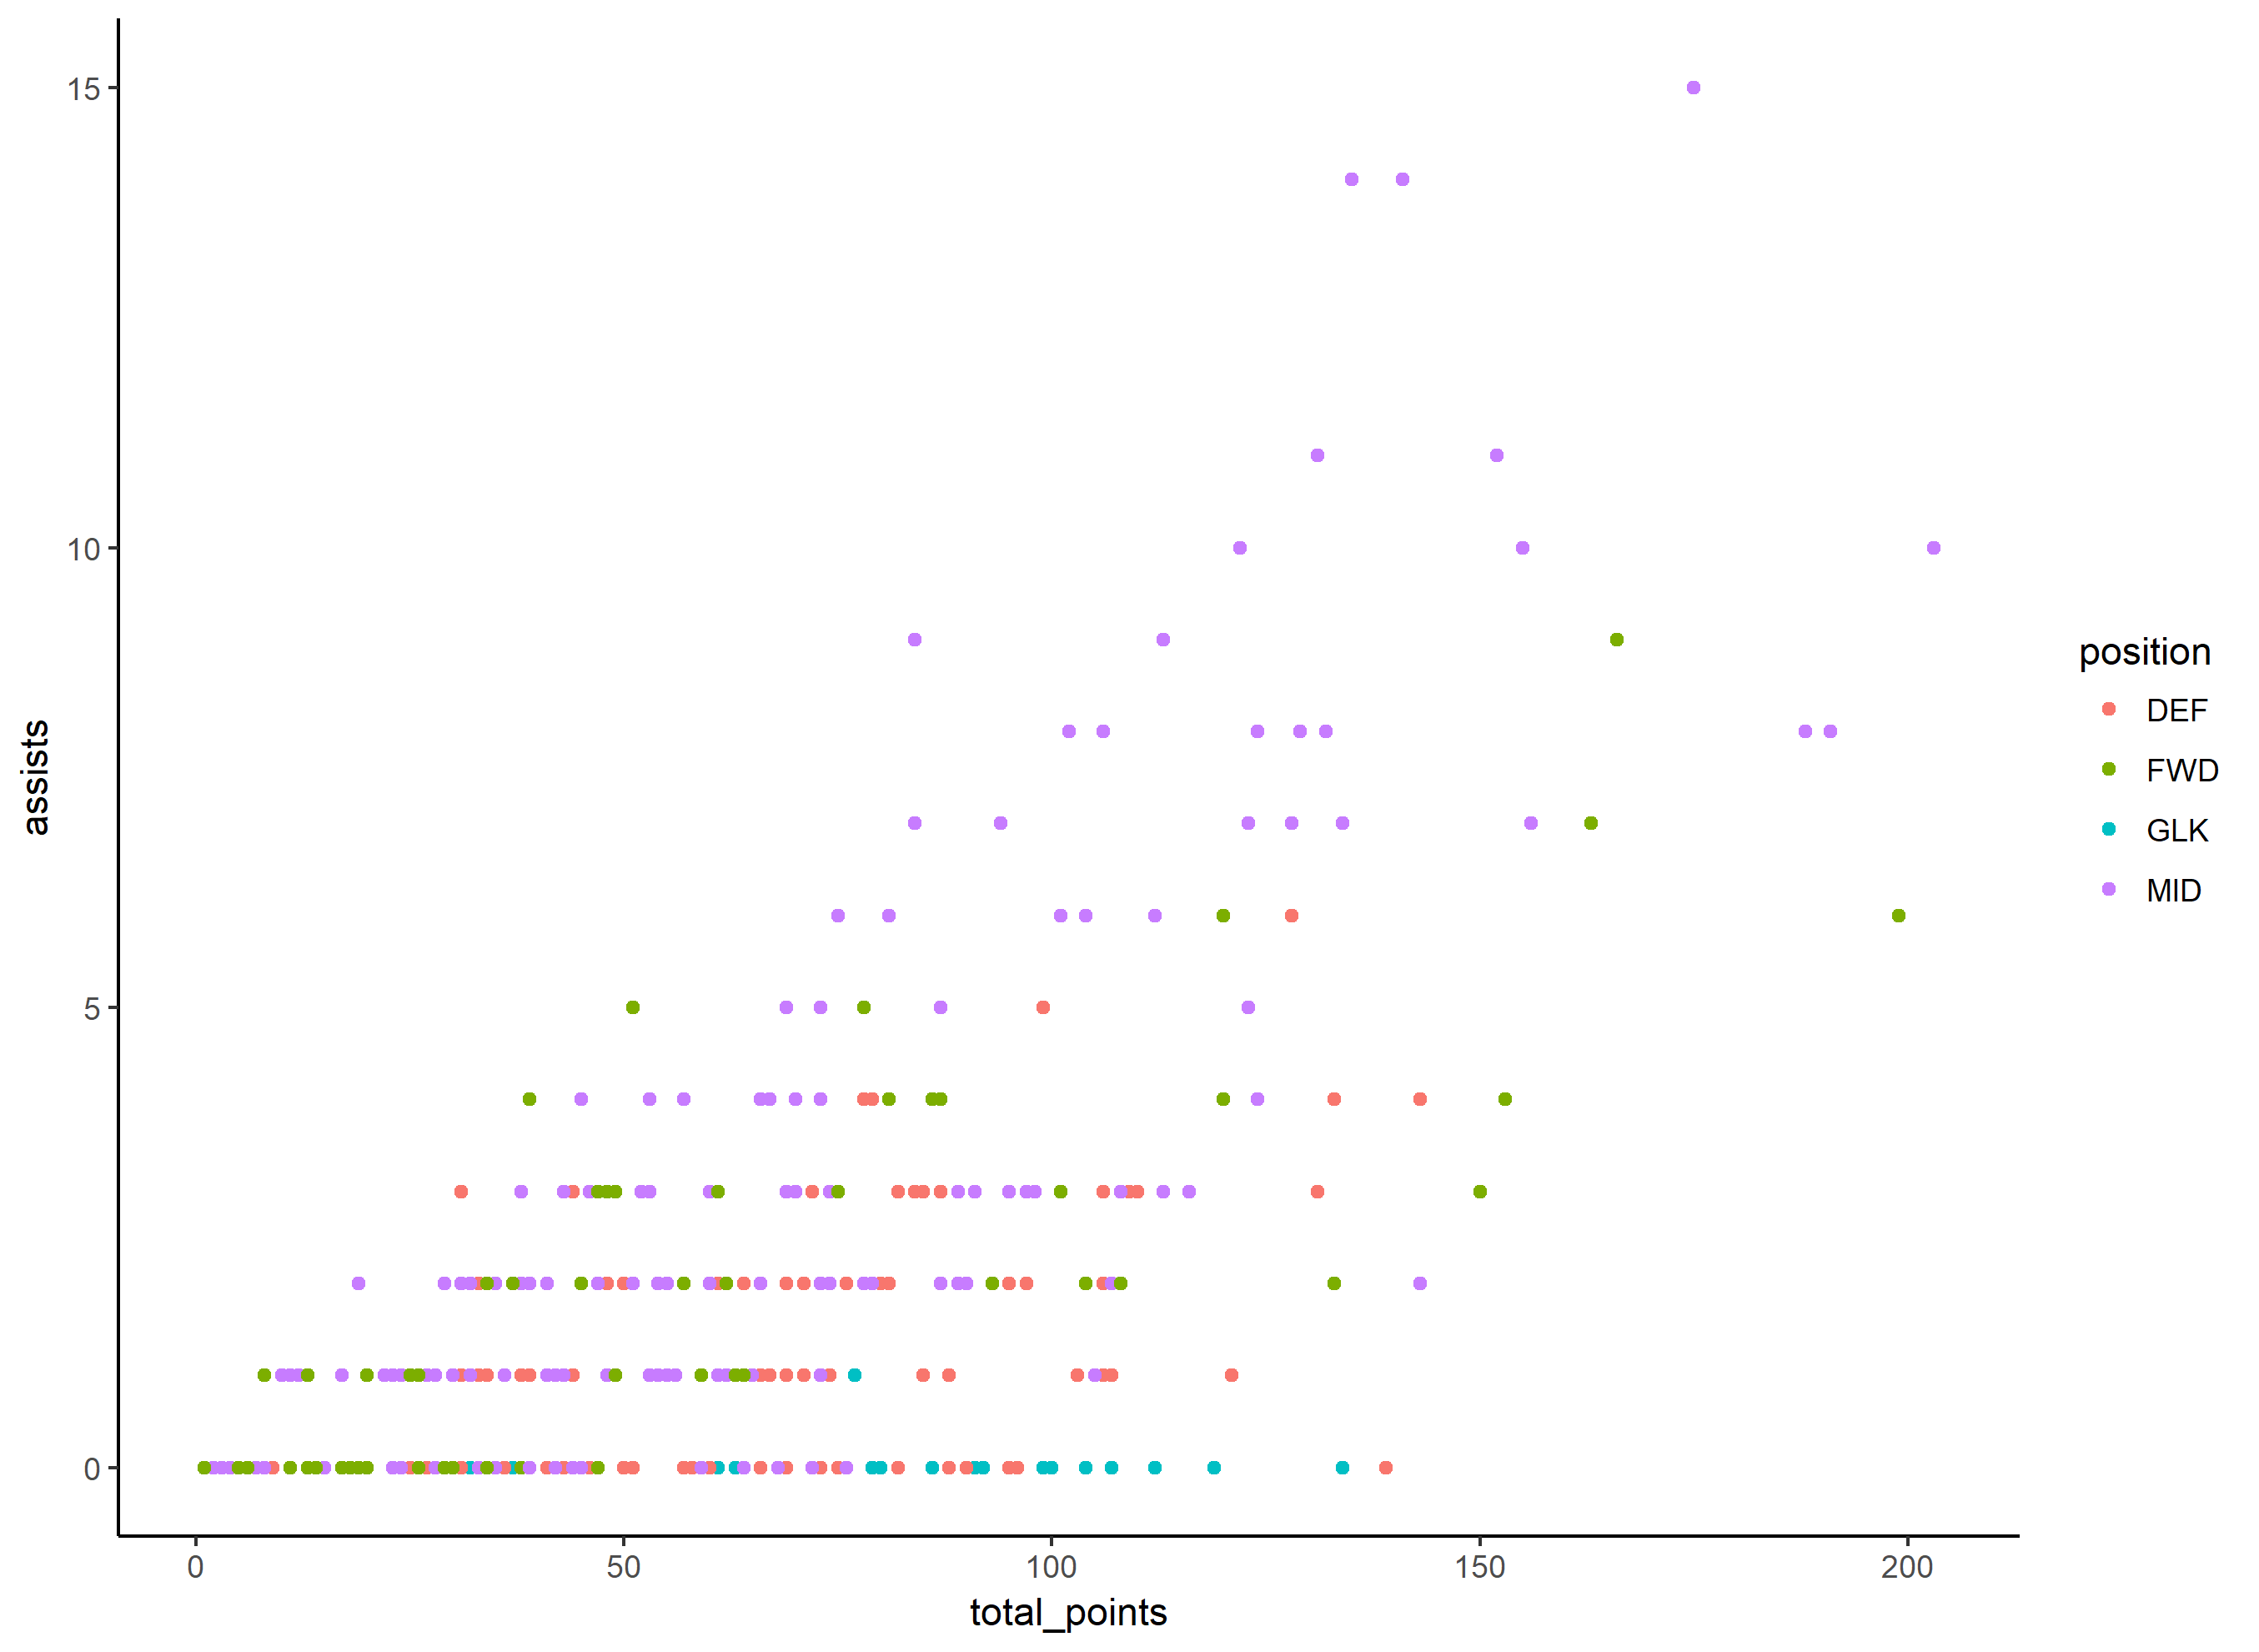
\includegraphics[width=.9\linewidth]{fig/chapter_6/assists_tot_poins.png}
  \caption{figure}{Time-series winter 16/17}
  \label{fig:assist_tot_p}
\end{minipage}
\end{figure}

\end{comment}

\begin{table}[H]
\centering
\begin{minipage}{.5\textwidth}
  \centering
  \captionsetup{justification=centering}
    \begin{figure}[H]
        \centering
        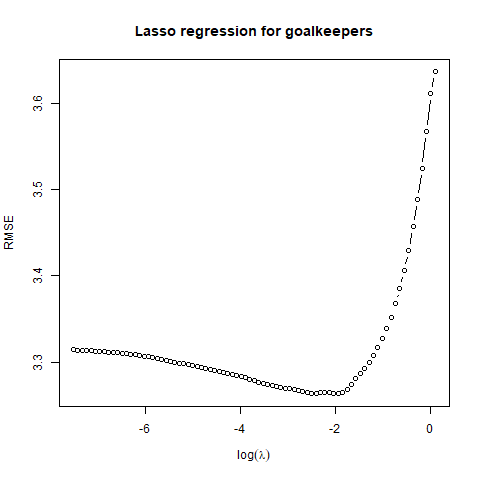
\includegraphics[scale=0.4]{fig/chapter_6/lasso_GLK.png}
    \end{figure}
    \captionof{figure}{RMSE for different values of $\lambda$ for goalkeepers}
    \label{fig:lasso_GLK_1}
\end{minipage}%
\begin{minipage}{.5\textwidth}
  \centering
  \captionsetup{justification=centering}
    \begin{tabular}{c}
    \\
    \textbf{Significant variables for Goalkeepers }\\
    \\
    \\
Opponent                              \\
Team                                  \\
Cost                                  \\
Transfers in                          \\
Transfers out                         \\
Home/Away                             \\
Minutes played                        \\
Saves                                 \\
Clean Sheets                          \\
Assists                               \\
Own Goals                            
    \\
    \\
    \\
    \\
\\


    \end{tabular}
\captionof{table}{Significant Variables for goalkeepers based on lasso regression and RMSE}
\label{tab:sig_var_GLK_1}
\end{minipage}
\end{table}

\begin{comment}
\textbf{Defenders}
In Figure \ref{fig:lasso_DEF} the RMSE of the test set is plotted against different values of $\lambda$. In Table \ref{tab:sig_var_DEF} the significant variables are listed
\end{comment}

\begin{comment}


\begin{table}[H]
\centering
\begin{minipage}{.5\textwidth}
  \centering
  \captionsetup{justification=centering}
    \begin{figure}[H]
        \centering
        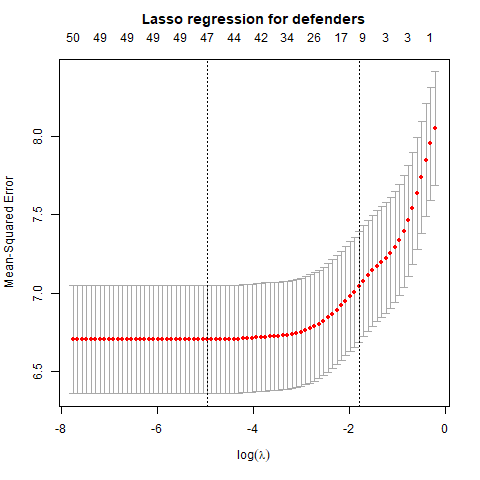
\includegraphics[scale=0.4]{fig/chapter_6/lasso_DEF.png}
    \end{figure}
    \captionof{figure}{RMSE for different values of $\lambda$ for defenders}
    \label{fig:lasso_DEF_1}
\end{minipage}%
\begin{minipage}{.5\textwidth}
  \centering
  \captionsetup{justification=centering}
    \begin{tabular}{c}
    \textbf{Significant variables for Defenders }\\
    \\
    \\
    \\
    
    Opponent                              \\
    Team                                  \\
    Cost                                  \\
    Transfers in                          \\
    Transfers out                         \\
    Home/Away                             \\
    Minutes played                        \\
    Yellow Cards                          \\
    Own Goals                             \\
    \\
    \\
    \\
    \\
   \\
   \\
    
    
    \end{tabular}
\captionof{table}{Significant Variables for midfielders based on lasso regression and RMSE}
\label{tab:sig_var_DEF_1}
\end{minipage}
\end{table}
\end{comment}
\begin{comment}


\begin{figure}[H]
    \centering
    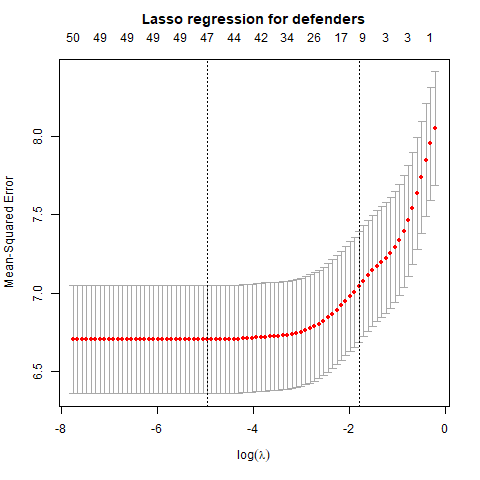
\includegraphics[scale=0.55]{fig/chapter_6/lasso_DEF.png}
    \caption{RMSE for different values of $\lambda$ for defenders}
\end{figure}

\begin{table}[H]
\centering
\caption{Significant Variables for defenders based on lasso regression and RMSE}
\begin{tabular}{l}
\textbf{Significant variables for Defenders }\\
Opponent                              \\
Team                                  \\
Cost                                  \\
Transfers in                          \\
Transfers out                         \\
Home/Away                             \\
Minutes played                        \\
Yellow Cards                          \\
Own Goals                                               
\end{tabular}
\end{table}

\end{comment}

\begin{comment}
\textbf{Midfielders}
In Figure \ref{fig:lasso_MID} the RMSE of the test set is plotted against different values of $\lambda$. In Table \ref{tab:sig_var_MID} the significant variables are listed
\end{comment}


\begin{table}[H]
\centering
\begin{minipage}{.5\textwidth}
  \centering
  \captionsetup{justification=centering}
    \begin{figure}[H]
        \centering
        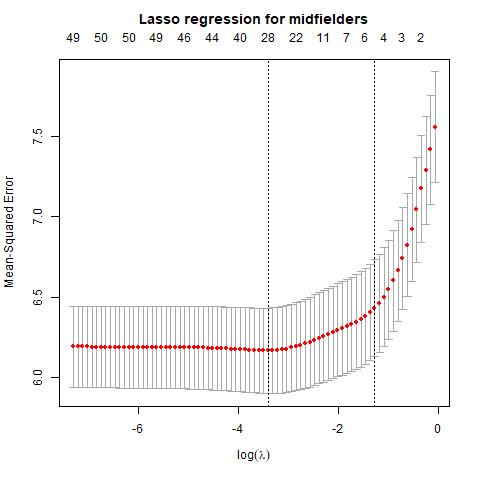
\includegraphics[scale=0.4]{fig/chapter_6/lasso_MID.png}
    \end{figure}
    \captionof{figure}{RMSE for different values of $\lambda$ for midfielders}
    \label{fig:lasso_MID_1}
\end{minipage}%
\begin{minipage}{.5\textwidth}
  \centering
  \captionsetup{justification=centering}
    \begin{tabular}{c}
    \\
    \textbf{Significant variables for Midfielders }\\
    \\
    \\
    \\
   Opponent                              \\
Team                                  \\
Cost                                  \\
Transfers in                          \\
Transfers out                         \\
Home/Away                             \\
Minutes played                        \\
Goals                                   \\
Penalty Misses                          \\
Clean Sheets                            \\
Assists                                 \\
\\
\\
\\

    \end{tabular}
\captionof{table}{Significant Variables for midfielders based on lasso regression and RMSE}
\label{tab:sig_var_MID_1}
\end{minipage}
\end{table}

\begin{comment}


\begin{figure}[H]
    \centering
    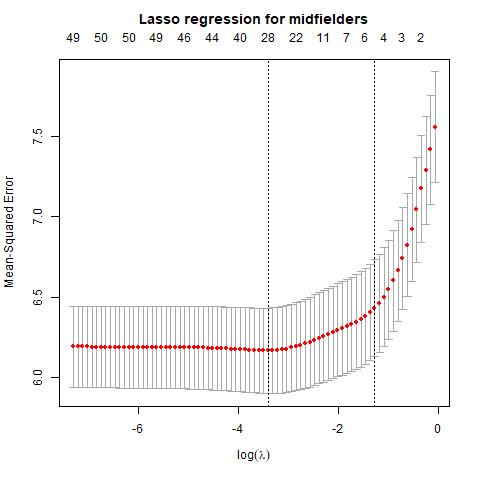
\includegraphics[scale=0.55]{fig/chapter_6/lasso_MID.png}
    \caption{RMSE for different values of $\lambda$ for midfielders}
\label{fig:lasso_MID}    
\end{figure}

\begin{table}[H]
\centering
\caption{Significant Variables for midfielders based on lasso regression and RMSE}
\label{tab:sig_var_MID}
\begin{tabular}{l}
\textbf{Significant variables for Midfielders }\\
Opponent                              \\
Team                                  \\
Cost                                  \\
Transfers in                          \\
Transfers out                         \\
Home/Away                             \\
Minutes played                        \\
Goals
        \\
Penalty Misses
        \\
Clean Sheets
        \\
Assists
\end{tabular}
\end{table}

\end{comment}

\begin{comment}
\textbf{Forwards}
In Figure \ref{fig:lasso_FWD} the RMSE of the test set is plotted against different values of $\lambda$. In Table \ref{tab:sig_var_FWD} the significant variables are listed
\end{comment}

\begin{table}[H]
\centering
\begin{minipage}{.5\textwidth}
  \centering
  \captionsetup{justification=centering}
    \begin{figure}[H]
        \centering
        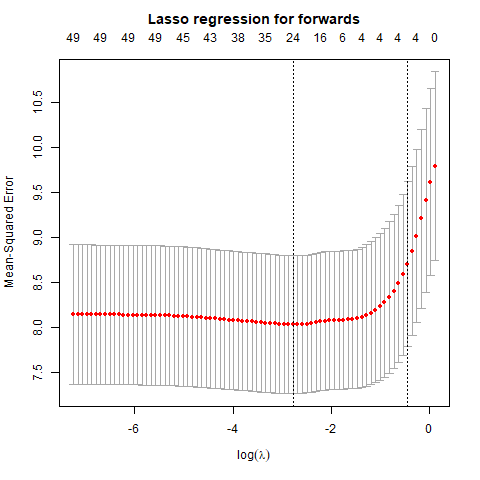
\includegraphics[scale=0.4]{fig/chapter_6/lasso_FWD.png}
    \end{figure}
    \captionof{figure}{RMSE for different values of $\lambda$ for forwards}
    \label{fig:lasso_FWD_1}
\end{minipage}%
\begin{minipage}{.5\textwidth}
  \centering
  \captionsetup{justification=centering}
    \begin{tabular}{c}
    \textbf{Significant variables for Forwards}\\
\\
\\    
\\
\\
Opponent                              \\
Team                                  \\
Cost                                  \\
Transfers in                          \\
Home/Away                             \\
Minutes played                        \\
Goals                                 \\
\\
\\
\\
\\
\\
\\
\\

 \end{tabular}
\captionof{table}{Significant Variables for forwards based on lasso regression and RMSE}
\label{tab:sig_var_FWD_1}
\end{minipage}
\end{table}

\begin{comment}

\begin{figure}[H]
    \centering
    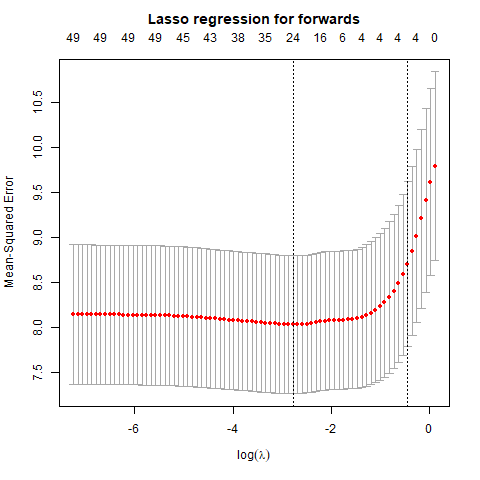
\includegraphics[scale=0.55]{fig/chapter_6/lasso_FWD.png}
    \caption{RMSE for different values of $\lambda$ for forwards}
\label{fig:lasso_FWD}    
\end{figure}

\begin{table}[H]
\centering
\caption{Significant Variables for forwards based on lasso regression and RMSE}
\label{tab:sig_var_FWD}
\begin{tabular}{l}
\textbf{Significant variables for Forwards}\\
Opponent                              \\
Team                                  \\
Cost                                  \\
Transfers in                          \\
Home/Away                             \\
Minutes played                        \\
Goals

\end{tabular}
\end{table}

\end{comment}